% Chapter 2

\chapter{Context and Objective} % Main chapter title

\label{Chapter2} % For referencing the chapter elsewhere, use \ref{Chapter2}

\lhead{Chapter 2. \emph{Context and Objective}} % This is for the header on each page - perhaps a shortened title
In this chapter, I will first introduce the context of this internship which is the Brain Computer Interface (BCI) and the new deep learning technique Domain Adaptation. From the problems identified for the EEG data, we propose the approach by using Domain Adaptation to eliminate the variabilty problem in the EEG data.

%----------------------------------------------------------------------------------------

\section{Context}


\subsection{BCI}{Brain Computer Interface}
Brain-computer interface is a method of communication based on neural activity generated by the brain and is independent of its normal output pathways of peripheral nerves and muscles. The neural activity used in BCI can be recorded using invasive or noninvasive techniques. The goal of BCI is not to determine a person's intent by eavesdropping on brain activity, but rather to provide a new channel of output for the brain that requires voluntary adaptive control by the user.\cite{wolpaw2000brain} The potential of BCI systems for helping handicapped people is obvious, the wheelchair controled by EEG signal is shown at \fref{fig:wheelchair}. There are several computer interfaces designed for disabled people.\cite{wickelgren2003brain} Most of these systems, however, require some sort of reliable muscular control such as neck, head, eyes, or other facial muscles. It is important to note that although requiring only neural activity, BCI utilizes neural activity generated voluntarily by the user. Interfaces based on involuntary neural activity, such as those generated during an epileptic seizure, utilize many of the same components and principles as BCI, but are not included in this field. BCI systems, therefore, are especially useful for severely disabled, or locked-in, individuals with no reliable muscular control to interact with their surroundings.

\begin{figure}[htbp]
	\centering
	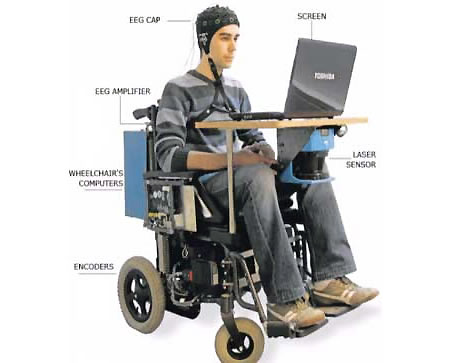
\includegraphics[width=10cm]{Figures/wheelchair.jpg}
	\caption[A wheelchair controled by EEG signal]{A wheelchair controled by EEG signal}
	\label{fig:wheelchair}
\end{figure}

But there's a main limitation for BCI is that the EEG data have a high inter-variability and intra-variability. EEG data are highly dependent on subject, so it requires to train the BCI on each subject. Also, it's highly dependent on session, EEG collected are varies from different time(like morning and evening), and even during a same work session, so it also requires to train on each subject for each session, which is difficult to realize and redundant. Thus we should find an approach to eliminate the subject-independent and session independent problem of EEG data.

\subsection{Domain Adaptation}
Top-performing deep architectures are trained on massive amounts of labeled data. In the absence of labeled data for a certain task, domain adaptation often provides an attractive option given that labeled data of similar nature but from a different domain (e.g. synthetic images) are available. The paper by [Ganin et al. 2015]\cite{ganin2014unsupervised} propose a new approach to domain adaptation in deep architectures that can be trained on large amount of labeled data from the source domain and large amount of unlabeled data from the target domain (no labeled target domain data is necessary).

As the training progresses, the approach promotes the emergence of “deep” features that are
\begin{enumerate}
	\item Discriminative for the main learning task on the source domain
	\item Invariant with respect to the shift between the domains.
\end{enumerate} 
The paper\cite{ganin2014unsupervised} shows that this adaptation behavior can be achieved in almost any feed-forward model by augmenting it with few standard layers and a simple new \textbf{gradient reversal layer}. The resulting augmented architecture can be trained using standard back-propagation. Overall, the approach can be implemented with little effort using any of the deep-learning packages. The method performs very well in a series of image classification experiments, achieving adaptation effect in the presence of big domain shifts and outperforming previous state-of-the-art on Office datasets.

\begin{figure}[htbp]
	\centering
	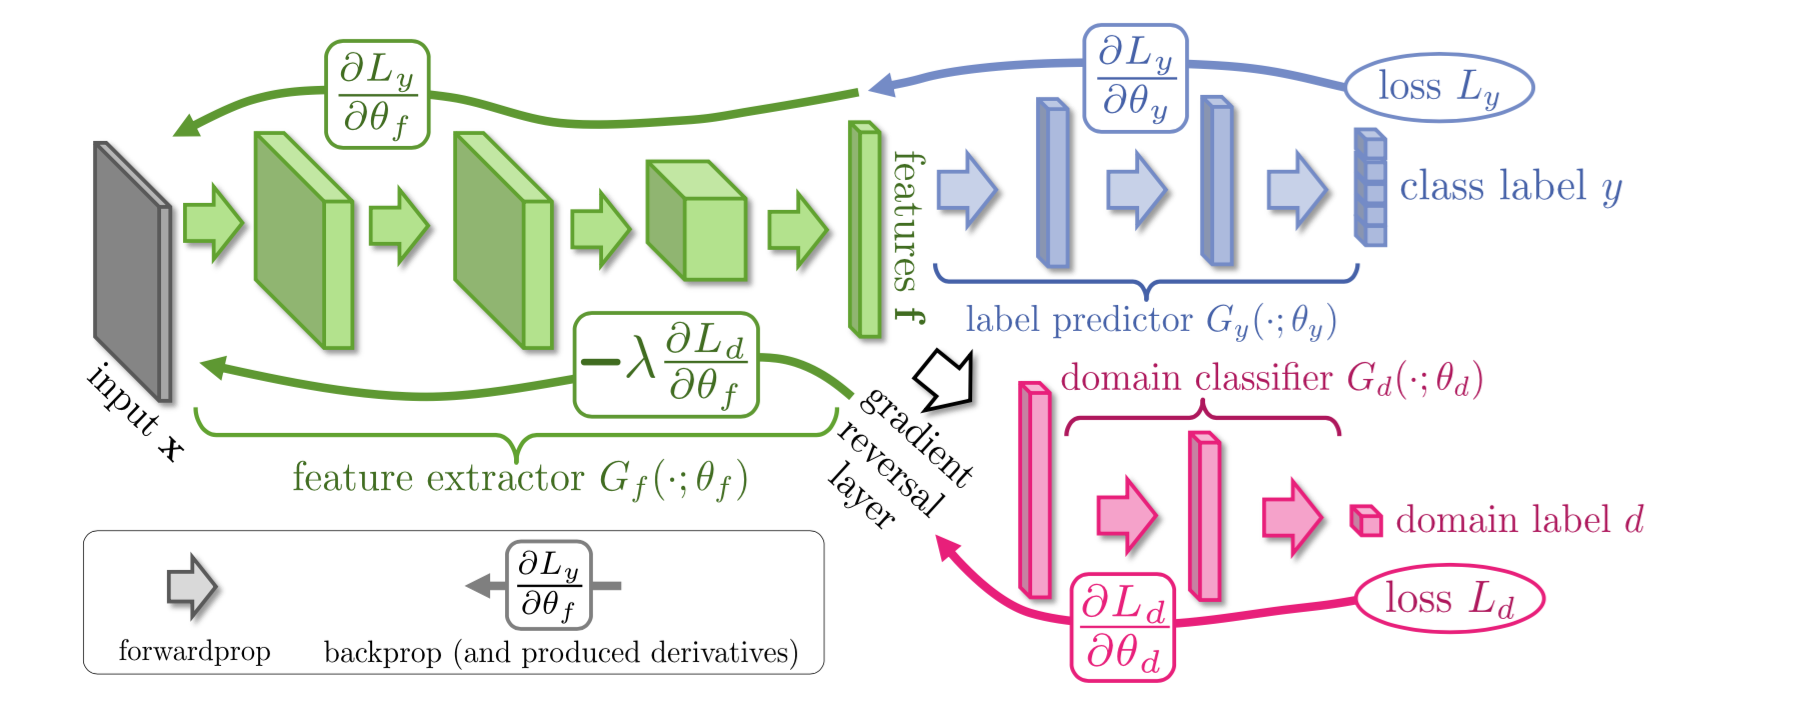
\includegraphics[width=15cm]{Figures/domainadaptation.png}
	\caption[Domain Adaptation Model Architecture]{Domain Adaptation Model Architecture}
	\label{fig:domainadaptation}
\end{figure}

This method involves two domains, the source domain and the target domain.  For example, the source domain can be MNIST dataset (handwritten digit database) and the target domain can be the SVHN dataset (The Street View House Numbers). Formally, the source is described through a training set, made of (instance, label) pairs:
\[ \mathcal{ S} = {(x_{i},y_{i}), x_{i} \in X, y_{i} \in Y, i \in [1,n]}  \]
where \textit{X} is the instance space (e.g. the vectors of pixel values) and \textit{Y} is the label space (e.g. the digit numbers). The target is described through a test set made of instances:
\[ \mathcal{T} = x'_{i}, x'_{i} \in X, i \in [1,n] \]
The general goal is to build a classifier \textit{h} for the source domain and for the target domain \textbf{without} gathering the target doamin labels.

The paper has proposed a model for the domain adaptation as \fref{fig:domainadaptation}. The proposed architecture includes a deep feature extractor (green) and a deep label predictor (blue), which together form a standard feed-forward architecture. Unsupervised domain adaptation is achieved by adding a domain classifier (red) connected to the feature extractor via a gradient reversal layer that multiplies the gradient by a certain negative constant during the backpropagationbased training. Otherwise, the training proceeds in a standard way and minimizes the label prediction loss (for source examples) and the domain classification loss (for all samples). Gradient reversal ensures that the feature distributions over the two domains are made similar (as indistinguishable as possible for the domain classifier), thus resulting in the domain-invariant features.

During the learning stage, we aim to minimize the label prediction loss on the annotated part (i.e. the source part) of the training set, and the parameters of both the feature extractor and the label predictor are thus optimized in order to minimize the empirical loss for the source domain samples. This ensures the discriminativeness of the features \textbf{f} and the overall good prediction performance of the combination of the feature extractor and the label predictor on the source domain. At the same time, we want to make the features \textbf{f} domain-invariant which is we want the representation of the two domains to be similar.

At training time, in order to obtain domain-invariant features, we seek the parameters of the feature mapping that maximize the loss of the domain classifier (by making the two feature distributions as similar as possible), while simultaneously seeking the parameters of the domain classifier that minimize the loss of the domain classifier. So as we can see, the parameter $\lambda$ of the Gradient Reversal Layer controls the trade-off between the two objectives that shape the features during learning.
%----------------------------------------------------------------------------------------

\section{Objective}
After the problem identified of the EEG data using in the BCI (high inter-variability and high intra-variability) .the objective of this internship thus is to build a subject-dependent, session-dependent representations of the EEG data. The sought representation must achieve a lossy compression of the signal to enabling the reconstruction of the brainwave data in order to further use in the BCI, besides, the representation of the signals gathered along different sessions follows the same distribution, or distribution as similar as possible. There's also a difficulty is that this reconstruction must preserve the complex spatio-temporal-frequency structure of the EEG data.




